%%%%%%%%%%%%%%%%%%%%%%%%%%%%%%%%%%%%%%%%%%%%%%

\part{\textsc{Matlab} and Solving Equations}

%%%%%%%%%%%%%%%%%%%%%%%%%%%%%%%%%

\chapter{Vectors, Functions, and  Plots in {\sc Matlab}}
\label{lec:vectors}

In these notes 
\begin{lstlisting}[frame=none,numbers=left,showlines=true]


\end{lstlisting}
will indicate commands to be entered 
at the {\sc Matlab} prompt \(\gg\) in the command window.
You do not type the symbol \(\gg\).

%%%%%%%%%%%%%

\subsection*{Entering vectors}

In \textsc{Matlab}, the basic objects are matrices, i.e.~arrays
of numbers. Vectors can be thought of as special matrices.
A row vector is recorded as a $1 \times n$ matrix
and a column vector is recorded as a $m \times 1$ matrix.
To enter a row vector in Matlab, type the following in the command window:
\begin{lstlisting}[frame=none,numbers=left]
v = [0 1 2 3]
\end{lstlisting}
and press enter. \textsc{Matlab} will print out the row vector.
To enter a column vector type
\begin{lstlisting}[frame=none,numbers=left]
u = [9; 10; 11; 12; 13]
\end{lstlisting}
You can access an entry in a vector with
\begin{lstlisting}[frame=none,numbers=left]
u(2)
\end{lstlisting}
and change the value of that entry with
\begin{lstlisting}[frame=none,numbers=left]
u(2)=47
\end{lstlisting}
You can extract a {\em slice}\ out of a vector with
\begin{lstlisting}[frame=none,numbers=left]
u(2:4)
\end{lstlisting}
You can change a row vector into a column vector, and vice versa,
easily in Matlab using
\begin{lstlisting}[frame=none,numbers=left]
w = v'
\end{lstlisting}
(This is called {\em transposing}\ the vector and we call \verb&'&
the transpose operator.)
There are also useful shortcuts to make vectors such as
\begin{lstlisting}[frame=none,numbers=left]
x = -1:.1:1
y = linspace(0,1,11)
\end{lstlisting}

%%%%%%%%%%%%%

\subsection*{Basic Formatting}

To make \textsc{Matlab} put fewer blank lines in its output, enter
\begin{lstlisting}[frame=none,numbers=left]
format compact
pi
x
\end{lstlisting}
To make \textsc{Matlab} display more digits, enter
\begin{lstlisting}[frame=none,numbers=left]
format long
pi
\end{lstlisting}
Note that this does not change the number of digits \textsc{Matlab} is
using in its calculations; it only changes what is displayed.

%%%%%%%%%%%%%%

\subsection*{Plotting Data}

Consider the data in Table~\ref{tab:viscosity}.\footnote{Adapted from
  Ayyup \&McCuen 1996, p.174.}
\begin{table}[h]
\centerline{
\begin{tabular}{|c|ccccc|}
\hline
 T ($\text{C}^\circ$)  & 5 & 20 & 30 & 50 & 55  \\
  $\mu$ & 0.08 & 0.015 & 0.009 & 0.006 & 0.0055 \\ \hline
\end{tabular}
}
\caption{Viscosity of a liquid as a function of temperature.}
\label{tab:viscosity}
\end{table}
We can enter this data into \textsc{Matlab} with the following
commands entered in the command window:
\begin{lstlisting}[frame=none,numbers=left]
x = [ 5  20  30  50  55 ]
y = [ 0.08  0.015  0.009  0.006  0.0055]
\end{lstlisting}
Entering the name of the variable retrieves its current values.
For instance
\begin{lstlisting}[frame=none,numbers=left]
x
y
\end{lstlisting}
We can plot data in the form of vectors using the plot command:
\begin{lstlisting}[frame=none,numbers=left]
plot(x,y)
\end{lstlisting}
This will produce a graph with the data points connected by lines.  If
you would prefer that the data points be represented by symbols
you can do so. For instance
\begin{lstlisting}[frame=none,numbers=left]
plot(x,y,'*')
plot(x,y,'o')
plot(x,y,'.')
\end{lstlisting}

%%%%%%%%%%%%%%%%

\subsection*{Data as a Representation of a Function}

A major theme in this course is that often we are interested
in a certain function $y = f(x)$, but the only
information we have about this function is a discrete set of data
$\{(x_i,y_i)\}$. Plotting the data, as we did above, can be thought of
envisioning the function using just the data. We will find later
that we can also do other things with the function, like
differentiating and integrating, just using
the available data. Numerical methods, the topic of this course,
means doing mathematics by computer. Since a computer can only store
a finite  amount of information, we will almost always be working
with a finite, discrete set of values of the function (data), rather
than a formula for the function.

%%%%%%%%%%%%%%%%

\subsection*{Built-in Functions}

If we wish to deal with formulas for functions, \textsc{Matlab} contains a
number of built-in functions, including all
the usual functions, such as \verb^sin( )^, \verb^exp( )^, etc.. The meaning
of most of these is clear. The dependent variable (input) always goes
in parentheses in \textsc{Matlab}. For instance
\begin{lstlisting}[frame=none,numbers=left]
sin(pi)
\end{lstlisting}
should return the value of $\sin \pi$, which is of course $0$ and
\begin{lstlisting}[frame=none,numbers=left]
exp(0)
\end{lstlisting}
will return $e^0$, which is $1$.
More importantly, the built-in functions  can operate
not only on single numbers but on vectors. For example
\begin{lstlisting}[frame=none,numbers=left]
x = linspace(0,2*pi,41)
y = sin(x)
plot(x,y)
\end{lstlisting}
will return a plot of $\sin x$ on the interval $[0,2 \pi]$

Some of the built-in functions in \textsc{Matlab} include:
\verb^cos( )^, \verb^tan( )^, \verb^sinh( )^, \verb^cosh( )^,
\verb^log( )^ (natural logarithm), \verb^log10( )^
(log base 10), \verb^asin( )^ (inverse sine), \verb^acos( )^, \verb^atan( )^.
To find out more about a function, use the \verb&help& command; try
\begin{lstlisting}[frame=none,numbers=left]
help plot
\end{lstlisting}

%%%%%%%%%%%%%%%%

\subsection*{User-Defined Anonymous Functions}

If we wish to deal with a function that is a combination of the
built-in functions, \textsc{Matlab} has a couple of ways for the user
to define functions.  One that we will use a lot is the anonymous
function, which is a way to define a function in the command window.
The following is a typical anonymous function:
\begin{lstlisting}[frame=none,numbers=left]
f = @(x) 2*x.^2 - 3*x + 1
\end{lstlisting}
This produces the function $f(x) = 2 x^2 -3x+1$. To obtain a single
value of this function enter
\begin{lstlisting}[frame=none,numbers=left]
y = f(2.23572)
\end{lstlisting}

Just as for built-in functions, the function $f$ as we defined it can
operate
not only on single numbers but on vectors. Try the following:
\begin{lstlisting}[frame=none,numbers=left]
x = -2:.2:2
y = f(x)
\end{lstlisting}
This is an example of {\em vectorization}, i.e.\ putting several
numbers into a vector and treating the vector all at once, rather than
one component at a time, and is one of the strengths of
\textsc{Matlab}.  The reason $f(x)$ works when $x$ is a vector is
because we represented $x^2$ by \verb&x.^2&. The \verb&.& turns the
exponent operator \verb&^& into entry-wise exponentiation, so that
\verb&[-2 -1.8 -1.6].^2& means $[(-2)^2, (-1.8)^2, (-1.6)^2]$ and
yields \verb&[4 3.24 2.56]&.  In contrast, \verb&[-2 -1.8 -1.6]^2&
means the matrix product $[-2, -1.8,-1.6][-2, -1.8,-1.6]$ and yields
only an error. The \verb&.& is needed in \verb&.^&, \verb&.*&, and
\verb&./&. It is not needed when you \verb&*& or \verb&/& by a scalar
or for \verb&+&.

The results can be plotted using the \verb&plot& command, just as for data:
\begin{lstlisting}[frame=none,numbers=left]
plot(x,y)
\end{lstlisting}
Notice that before plotting the function, we in effect converted it
into data. Plotting on any machine always requires this step.


%%%%%%%%%%%%%%%%

\section*{Exercises}
\begin{list}
{\arabic{chapter}.\arabic{exercise}}{\usecounter{exercise}}

\item Recall that \verb&.*&, \verb&./&, \verb&.^& are component-wise operations.
Make row vectors $\mathbf{a} = 0:1:3$ and $\mathbf{b} = [-1 \  \ 0 \  \ 1 \  \ 2]$.
Try the following commands and report the answer (or error) they produce. Are any of the results surprising?

(a)  \verb&a.*b&, \hspace{.2in}    (b)  \verb&a*b&, \hspace{.2in}  (c)  \verb&a*b'&, \hspace{.2in}  (d)  \verb&a+3*b&,  

(e)   \verb&a./b&, \hspace{.2in}    (f)  \verb&2*b./a&,   \hspace{.2in}  (g)  \verb&a.^3&, \hspace{.2in}  (h) \verb&a.^b&,


\item Find a table of data in an engineering or science textbook or 
  website. Input it as vectors and plot it, {\em using symbols at the data points}. 
  
  Use the insert icon to
  label the axes and add a title to your graph. Turn in the graph.
  Indicate what the data is and properly reference where it came from.
  
\item  Find a {\em non-linear} function formula in an engineering or science textbook or 
  website. Make an anonymous function that produces that function. Plot it
  with a {\em smooth curve}  on a physically relevant  domain. 
  
  Label the axes and add a title to your
   graph. Turn in the graph and include the Matlab command for 
   the anonymous function. Indicate what the function means and properly 
   reference where it came from.
   


\end{list}






%%%%%%%%%%%%%%%%%%%%%%%%%%%%%%%%%%%%%%%%%%%%%%%%%%%%%%%%%%%%%%%%%%%%%%%%%%%%

\chapter{{\sc  Matlab} Programs}

In \textsc{Matlab}, programs may be written and saved in files with
a suffix \verb&.m& called {\em M-files}. There are two types of
M-file programs: {\em functions} and {\em scripts}.

%%%%%%%%%%%%%%

\subsection*{Function Programs}

Begin by clicking on the new document icon in the top
left of the \textsc{Matlab} window (it looks like an empty sheet of paper).

In the document window type the following:
\begin{lstlisting}
function y = myfunc(x)
    y = 2*x.^2 - 3*x + 1;
end
\end{lstlisting}

Save this file as: \verb&myfunc.m& in your working directory.
This file can now be used in the command window just like any
predefined Matlab function; in the command window enter:
\begin{lstlisting}[frame=none,numbers=left]
x = -2:.1:2;     % Produces a vector of x values
y = myfunc(x);   % Produces a vector of y values
plot(x,y)
\end{lstlisting}
Note that the fact we used \verb&x& and \verb&y& in both the function
program and in the command window was just a coincidence. In fact, it
is the name of the file \verb&myfunc.m& that actually mattered, not
what anything in it was called.
We could just as well have made the function
\begin{lstlisting}
function nonsense = yourfunc(inputvector)
    nonsense = 2*inputvector.^2 - 3*inputvector + 1;
end
\end{lstlisting}

Look back at the program.
All function programs are like this one, the essential elements are:
\begin{itemize}
\item Begin with the word \verb&function&.
\item There is an input and an output.
\item The output, name of the function and the input must appear in the first line.
\item The body of the program must assign a value to the output variable(s). 
\item The program cannot access variables in the current workspace unless they
           are input.
\item Internal variables inside a function do not appear in the current workspace.
\end{itemize}

Functions can have multiple inputs, which are separated by commas. 
For example:
\begin{lstlisting}
function y = myfunc2d(x,p)
    y = 2*x.^p - 3*x + 1;
end
\end{lstlisting}

Functions can have multiple outputs, which are collected into a vector. 
Open a new document and type:
\begin{lstlisting}
function [x2 x3 x4] = mypowers(x)
    x2 = x.^2;
    x3 = x.^3;
    x4 = x.^4;
end
\end{lstlisting}
Save this file as \verb&mypowers.m&.
In the command window, we can use the results of the program to make graphs:
\begin{lstlisting}[frame=none,numbers=left]
x = -1:.1:1
[x2 x3 x4] = mypowers(x);
plot(x,x,'black',x,x2,'blue',x,x3,'green',x,x4,'red')
\end{lstlisting}

\subsubsection{Printing, Returning, Capturing, and Printing}

Notice that in the examples above, lines ending with a semicolon ``;''
did not print their results.

Try the following:
\begin{lstlisting}[frame=none,numbers=left]
myfunc(3)
ans^2
\end{lstlisting}
Although \verb&myfunc& returned a value, we did not capture it. By
default \textsc{Matlab} captured it as \verb&ans& so we can use it in
our next computation. However, \textsc{Matlab} always uses \verb&ans&
(for answer), so the result is likely to get overwritten.

Then try:
\begin{lstlisting}[frame=none,numbers=left]
z = 0
z = myfunc(2)
z^2
\end{lstlisting}
\verb&myfunc&
returned a value that it internally called \verb&y& and we captured
the result in \verb&z&. We can now use \verb&z& for other calculations.

Now make a program 
\begin{lstlisting}
function myfuncnoreturn(x)
    y = 2*x.^2 - 3*x + 1
end
\end{lstlisting}
and try:
\begin{lstlisting}[frame=none,numbers=left]
myfuncnoreturn(4)
ans^2
y^2
\end{lstlisting}
Although the value of \verb&y& was printed within the function, it was
not returned, so neither the value of \verb&y& nor the value of
\verb&ans& was changed. Thus we cannot use the result from the function.

In general, the best way to use a function is to capture the result
it returns and then use or print this result.
Printing within functions is bad form; however, for
understanding what is happening within a function it is useful to print, so many
functions in this book do print.


%%%%%%%%%%%%%%%%

\subsection*{Script Programs}

\textsc{Matlab} uses a second type of program that differs from
a function program in several ways, namely:
\begin{itemize}
\item There are no inputs and outputs.
\item A script program may use, create  and change variables in the current
  workspace (the variables used by the command window).
\end{itemize}
Below is a script program that accomplishes the same thing as
the function program plus the commands in the previous section:
\begin{lstlisting}
x2 = x.^2;
x3 = x.^3;
x4 = x.^4;
plot(x,x,'black',x,x2,'blue',x,x3,'green',x,x4,'red')
\end{lstlisting}

Type this program into a new document and save it as \verb&mygraphs.m&.
In the command window enter:
\begin{lstlisting}[frame=none,numbers=left]
x = -1:.1:1;
mygraphs
\end{lstlisting}
Note that the program used the variable \verb&x& in its calculations, even
though \verb&x& was defined in the command window, not in the program.

Many people use script programs for routine calculations that
would require typing more than one
command in the command window. They do this because correcting
mistakes is easier in a program than in the command window.

%%%%%%%%%%%%%%%%

\subsection*{Program Comments}

For programs that have more than a couple of lines it
is important to include comments. Comments allow other
people to know what your program does and they also
remind yourself what your program does if you set it
aside and come back to it later. It is best to include
comments not only at the top of a program, but also
with each section. In \textsc{Matlab} anything that
comes in a line after a \verb&%& 
is a comment.

For a function program, the comments should at least give the purpose,
inputs, and outputs. A properly commented version of the function with
which we started this section is:
\begin{lstlisting}
function y = myfunc(x)
    % Computes the function 2x^2 -3x +1
    % Input: x -- a number or vector; 
    %             for a vector the computation is elementwise
    % Output: y -- a number or vector of the same size as x
    y = 2*x.^2 - 3*x + 1;
end
\end{lstlisting}

For a script program, there should be an initial comment stating the purpose of the script.
It is also  helpful to include the name of the program at the beginning.
For example:
\begin{lstlisting}
% mygraphs
% plots the graphs of x, x^2, x^3, and x^4
% on the interval [-1,1]

% fix the domain and evaluation points
x = -1:.1:1;

% calculate powers
% x1 is just x
x2 = x.^2;
x3 = x.^3;
x4 = x.^4;

% plot each of the graphs
plot(x,x,'+-',x,x2,'x-',x,x3,'o-',x,x4,'--')
\end{lstlisting}

The \textsc{Matlab} command \verb&help& prints the first block of
comments from a file. If we save the above as \verb&mygraphs.m& and
then do
\begin{lstlisting}[frame=none,numbers=left]
help mygraphs
\end{lstlisting}
it will print into the command window:
\begin{lstlisting}[frame=none,numbers=left]
mygraphs
plots the graphs of x, x^2, x^3, and x^4
on the interval [-1,1]
\end{lstlisting}

%%%%%%%%%%%%%%%%

\section*{Exercises}

\begin{list}
{\arabic{chapter}.\arabic{exercise}}{\usecounter{exercise}}
\item Write a well-commented {\bf function} program for the function
  $x^2 e^{-x^2}$, using component-wise operations (such as \verb&.*&
  and~\verb&.^&). To get $e^x$ use \verb&exp(x)&.  Plot the function
  on $[-5,5]$ using enough points to make the graph smooth. Turn in
  the program and the graph.
%(The graph of
%      the function $e^{-x^2}$ is the bell-curve that is used
%      in probability and statistics.)

\item Write a well-commented {\bf script} program that graphs the
  functions $\sin x$, $\sin 2x$, $\sin 3x$, $\sin 4x$, $\sin 5x$ and
  $\sin 6x$ on the interval $[0, 2\pi]$ on one plot. ($\pi$ is
  \verb&pi& in \textsc{Matlab}.) Use a sufficiently small step size to
  make all the graphs smooth. 
  Turn in the program and the graph.
\end{list}





%%%%%%%%%%%%%%%%%%%%%%%%%%%%%%%%%%%%%%%%%%%%%%%%


\chapter{Newton's Method and Loops}
\label{lec:newton}

%%%%%%%%%%%%%%%%

\subsection*{Solving equations numerically}

For the next few lectures we will focus on the problem of solving an
equation:
\begin{equation}\label{fzero}
     f(x) = 0.
\end{equation}
As you learned in calculus, the final step in many optimization
problems is to solve an equation of this form where $f$ is the
derivative of a function, $F$, that you want
to maximize or minimize. In real engineering problems the
functions, $f$, you wish to find roots for can come from a large variety of
sources, including formulas, solutions of differential equations, experiments,
or simulations.


%%%%%%%%%%%%%%%%

\subsection*{Newton iterations}

We will denote an actual solution of equation (\ref{fzero}) by $x^*$.
There are three methods that you may have discussed in Calculus:
the bisection method, the secant method and Newton's method. All
three depend on beginning close (in some sense) to an actual solution
$x^*$.

Recall Newton's method. You should know that the basis for
Newton's method is approximation of a function by its linearization
at a point, i.e.
\begin{equation}\label{linapp}
f(x) \approx f(x_0) + f'(x_0)(x-x_0).
\end{equation}
Since we wish to find $x$ so that $f(x) =0$, set the left hand side ($f(x)$)
of this approximation equal to $0$ and solve for $x$ to obtain:
\begin{equation}\label{newtona}
x \approx x_0 - \frac{f(x_0)}{f'(x_0)}.
\end{equation}
We begin the method with the initial guess
$x_0$, which we hope is fairly close to $x^*$.
Then we define a sequence of points $\{x_0, x_1, x_2, x_3, \ldots \}$
from the formula:
\begin{equation}\label{newton}
x_{i+1} = x_i - \frac{f(x_i)}{f'(x_i)},
\end{equation}
which comes from (\ref{newtona}).
If $f(x)$ is reasonably well-behaved near $x^*$ and $x_0$ is
close enough to $x^*$, then it is a fact that the sequence will
converge to $x^*$ and will do it very quickly.


%%%%%%%%%%%%%%%%

\subsection*{The loop: \texttt{for ... end}}

In order to do Newton's method, we need to repeat the
calculation in (\ref{newton}) a number of times. This
is accomplished in a program using a {\em loop}, which
means a section of a program which is repeated. The simplest
way to accomplish this is to count the number of times
through. In \textsc{Matlab}, a \verb&for ... end& statement makes a loop
as in the following simple function program:
\begin{lstlisting}
    % mysum
    % Gives the sum of the first n integers   
    %
    n = 100            
    S = 0;            % start at zero
    % The loop:
    for i = 1:n       % do n times
        S = S + i;    % add the current integer
    end               % end of the loop
    S
\end{lstlisting}

Save this program as a {\bf script} named \verb& mysum & and
run it by typing \verb& mysum & in the command window.
The result will be the sum of the first 100 integers.
Next change $n$ to 1,000,000 and run the program again.

All \verb&for ... end& loops have the same format, it begins
with \verb&for&, followed by an index (\verb&i&) and a range of numbers
(\verb&1:n&). Then
come the commands that are to be repeated. Last comes
the \verb&end& command.

Loops are one of the main ways that computers are made
to do calculations that humans cannot. Any calculation
that involves a repeated process is easily done by
a loop.

Now let's do a program that does n steps (iterations)
of Newton's method.
We will need to input the function, its derivative, the initial
guess, and the number of steps. The output will be the final
value of $x$, i.e.~$x_n$. If we are only interested in the
final approximation, not the intermediate steps, which is
usually the case in the real world, then we can use a single
variable \verb&x& in the program \programlink{mynewton.m} and change it at each step:
\lstinputlisting{../programs/mynewton.m}

In the command window set to print more digits via
\begin{lstlisting}[frame=none,numbers=left]
format long
\end{lstlisting}
and to not print blank lines via
\begin{lstlisting}[frame=none,numbers=left]
format compact
\end{lstlisting}
Then define a function: $f(x) = x^3 - 5$
i.e.
\begin{lstlisting}[frame=none,numbers=left]
f = @(x) x^3 - 5
\end{lstlisting}
and define $f1$ to be its derivative, i.e.
\begin{lstlisting}[frame=none,numbers=left]
f1 = @(x) 3*x^2
\end{lstlisting}
Then run \verb&mynewton& on this function.
By trial and error, what is the lowest value of \verb&n& for which the
program converges (stops changing).  By simple algebra, the true root
of this function is $\sqrt[3]{5}$. How close is the program's answer
to the true value?

%%%%%%%%%%%%

\subsection*{Convergence}

Newton's method converges rapidly when $f'(x^*)$ is nonzero and
finite, and $x_0$ is close enough to $x^*$ that the  linear approximation
(\ref{linapp}) is valid.
Let us take a look at what can go wrong.

For $f(x)=x^{1/3}$ we have $x^*=0$ but $f'(x^*)=\infty$.  If you try
\begin{lstlisting}[frame=none,numbers=left]
f = @(x) x^(1/3)
f1 = @(x) (1/3)*x^(-2/3)
x = mynewton(f,f1,0.1,10)
\end{lstlisting}
then $x$ explodes.

For $f(x)=x^2$ we have $x^*=0$ but $f'(x^*)=0$.  If you try
\begin{lstlisting}[frame=none,numbers=left]
f = @(x) x^2
f1 = @(x) 2*x
x = mynewton(f,f1,1,10)
\end{lstlisting}
then $x$ does converge to $0$, but not that rapidly.

If $x_0$ is not close enough to $x^*$ that the linear approximation
(\ref{linapp}) is valid, then the iteration (\ref{newton}) gives some
$x_1$ that may or may not be any better than $x_0$. If we keep iterating,
then either
\begin{itemize}
\item
$x_n$ will eventually get close to $x^*$ and the method will then
converge (rapidly), or
\item
the iterations will not approach $x^*$.
\end{itemize}
%
%To see the second case try:\\
%\verb& > f = inline('x^(1/3) - 1')&\\
%\verb& > f1 = inline('(1/3)*x^(-2/3)')&\\
%The obvious solution of $x^{1/3} - 1 = 0$ is $1$.
%If we try $x_0$ close to $1$, the program will produce
%the correct answer in only a few steps.\\
%\verb& > x = mynewton(f,f1,2,10)&\\
%If, however, you choose $x_0$ far from $1$ even a large number of
%iterations will not produce the desired result:\\
%\verb& > x = mynewton(f,f1,10,10)&


%%%%%%%%%%%%%%%%%%%%%%%
\newpage
\subsection*{Exercises}

\nobreak \begin{list}
{\arabic{chapter}.\arabic{exercise}}{\usecounter{exercise}}


   
\item Enter: \verb&format long&.  Use \programlink{mynewton.m} on the function
  $f(x) = x^5 - 2$, with $x_0 = 1$. By trial and error, what is the
  lowest value of \verb&n& for which the program converges (stops
  changing). Compute the error, which is how close the program's
  answer is to the true value. Compute the residual, which is the
  program's answer plugged into $f$. (See the next section for discussion.) 
  Are the error and residual zero?
   
\item For $f(x) = x^2 - 5$, perform 3 iterations of Newton's method
  with starting point $x_0 = 2$. (By hand, but use a calculator.) Show all
  steps.
  Calculate the solution ($x^* = \sqrt{5}$) on a calculator and find
  the errors and percentage errors of $x_0$, $x_1$, $x_2$ and $x_3$.
  Use enough digits so that you do not falsely conclude the error is
  zero. 
  \label{exr:newtonbyhand}


\item Suppose a ball is dropped from a height of 3 meters onto a hard
  surface and the coefficient of restitution of the collision is .91
  (see Wikipedia for an explanation).  Write a well-commented {\bf
    script} program to calculate the total distance the ball has
  traveled when it hits the surface for the \verb&n&-th time.  Enter:
  \verb&format long&. By trial and error approximate how large
  \verb&n& must be so that total distance stops changing. Turn in the
  program and a brief summary of the results. (This program does not
  use Newton's method. It should be modeled on \verb&mysum.m&.)
  \label{exr:bounce}


\end{list}




%%%%%%%%%%%%%%%%%%%%%%%%%%%%%%%%%%%%%%%%%%%%%%%%%%%%%%%%%%%%%%%

\chapter{Controlling Error and Conditional Statements}

%%%%%%%%%%%%%%%%

\subsection*{Measuring error and the Residual}

If we are trying to find a numerical solution of an equation
$f(x) = 0$, then there are a few different ways we can measure
the error of our approximation. The most direct way to
measure the error would be as
$$
   \{ \text{Error at step $n$} \} = e_n = x_n - x^*
$$
where $x_n$ is the $n$-th approximation and $x^*$ is the true
value. However, we usually do not know the value of $x^*$, or
we wouldn't be trying to approximate it. This makes
it impossible to know the error directly, and so we must be
more clever.

One possible strategy, which often works,  is to
run a program until the approximation $x_n$ stops changing.
The problem with this is that it sometimes doesn't work. Just because the
program stop changing does not necessarily mean that $x_n$ is
close to the true solution.

For Newton's method we have the following principle:
{\bf At each step the number of significant digits roughly
doubles.}
While this is an important statement about the error
(since it means Newton's method
converges really quickly), it is somewhat hard to use in a
program.

Rather than measure how close $x_n$ is to $x^*$, in this and many other
situations it is much more practical to measure how close the equation
is to being satisfied, in other words, how close $y_n = f(x_n)$ is to $0$.
We will use the quantity $r_n =  f(x_n)-0$, called the {\em residual},
in many different situations. Most of the time we only care about the
size of $r_n$, so we use the absolute value of the residual as a measure
of how close the solution is to solving the problem:
$$
  |r_n|=|f(x_n)|.
$$



%%%%%%%%%%%%%%%%

\subsection*{The \texttt{if ... end} statement}

If we have a certain tolerance
for $|r_n| = |f(x_n)|$, then we can incorporate that into our Newton method
program using an \verb&if ... end& statement:
\begin{lstlisting}
function x = mynewton(f,f1,x0,n,tol)
    % Solves f(x) = 0 by doing n steps of Newton's method starting at x0.
    % Inputs: f -- the function
    %         f1 -- it's derivative
    %         x0 -- starting guess, a number
    %         tol -- desired tolerance, prints a warning if |f(x)|>tol
    % Output: x -- the approximate solution
    x = x0;                   % set x equal to the initial guess x0
    for i = 1:n               % Do n times
        x = x - f(x)/f1(x)  % Newton's formula
    end
    r = abs(f(x))
    if r > tol
        warning('The desired accuracy was not attained')
    end
end
\end{lstlisting}


In this program \verb&if& checks if \verb&abs(y) > tol&
is true or not. If it is true then it does everything
between there and \verb&end&. If not true, then it skips
ahead to \verb&end&.

In the command window define a function and its derivative:
\begin{lstlisting}[frame=none,numbers=left]
f = @(x) x^3-5
f1 = @(x) 3*x^2
\end{lstlisting}
Then use the program with $n=3$, $tol = .01$, and $x_0=2$.
Next, change $tol$ to $10^{-10}$ and repeat.

%%%%%%%%%%%%%%%%

\subsection*{The loop: \texttt{while ... end}}

While the previous program will tell us if it worked or not,
we still have to input \verb&n&, the number of steps to take.
Even for a well-behaved problem, if we make \verb&n& too small
then the tolerance will not be attained and we will have to
go back and increase it, or, if we make \verb&n& too big, then
the program will take more steps than necessary.

One way to control the number of steps taken is to iterate
until the residual $|r_n| = |f(x)| = |y|$ is small enough.
In \textsc{Matlab} this is easily accomplished with a
\verb&while ... end& loop.
\begin{lstlisting}
function x = mynewtontol(f,f1,x0,tol)
    % Solves f(x) = 0 using Newton's method until |f(x)| < tol.
    % Inputs: f -- the function
    %         f1 -- it's derivative
    %         x0 -- starting guess, a number
    %         tol -- desired tolerance, runs until |f(x)|<tol
    % Output: x -- the approximate solution
    x = x0;                   % set x equal to the initial guess x0
    y = f(x);
    while abs(y) > tol     % Do until the tolerence is reached.
        x = x - y/f1(x)    % Newton's formula
        y = f(x)
    end
end
\end{lstlisting}


The statement \verb&while ... end& is a loop,
similar to \verb&for ... end&, but instead of going through the
loop a fixed number of times it keeps going as long as the statement
\verb&abs(y) > tol & is true.

One obvious drawback of the program is that \verb&abs(y)& might
never get smaller than \verb&tol&. If this happens, the program
would continue to run over and over until we stop it. Try this
by setting the tolerance to a really small number:
\begin{lstlisting}[frame=none,numbers=left]
tol = 10^(-100)
\end{lstlisting}
then run the program again for $f(x) = x^3 - 5$.
(You can use \verb&Ctrl-c& to stop a program when it is stuck.)

One way to avoid an infinite loop is add a counter variable, say
\verb& i & and a maximum number of iterations to the programs.
Using the \verb& while & statement, this can be accomplished as:
\begin{lstlisting}
function x = mynewtontol(f,f1,x0,tol)
    % Solves f(x) = 0 using Newton's method until |f(x)| < tol.
    %     Safety stop after 1000 iterations
    % Inputs: f -- the function
    %         f1 -- it's derivative
    %         x0 -- starting guess, a number
    %         tol -- desired tolerance, runs until |f(x)|<tol 
    % Output: x -- the approximate solution
    x = x0;    % set x equal to the initial guess x0. 
    i=0;       % set counter to zero 
    y = f(x);
    while abs(y) > tol & i < 1000  
        % Do until the tolerence is reached or max iter.
        x = x - y/f1(x)    % Newton's formula
        y = f(x)
        i = i+1;           % increment counter
    end
end
\end{lstlisting}


\newpage
%%%%%%%%%%%%%%%%

\subsection*{Exercises}

\nobreak
\begin{list}
{\arabic{chapter}.\arabic{exercise}}{\usecounter{exercise}}

\item In Calculus we learn that a geometric series has an exact sum
$$
   \sum_{i=0}^\infty r^i = \frac{1}{1-r}
   \,,
$$
provided that $|r|<1$. For instance, if $r = .5$ then the sum is
exactly $2$.  Below is a script program that lacks one line as
written.  Put in the missing command and then use the program to
verify the result above. How many steps does it take? How close is the
answer to $2$?
\begin{lstlisting}
% Computes a geometric series until it seems to converge
format long
format compact
r = .5;
Snew = 0;           % start sum at 0
Sold = -1;          % set Sold to trick while the first time
i = 0;              % count iterations
while Snew > Sold   % is the sum still changing?
   Sold = Snew;     % save previous value to compare to
   Snew = Snew + r^i;
   i=i+1;
Snew                % prints the final value.
i                   % prints the # of iterations.
\end{lstlisting}
Add a line at the end of the program to compute the error of
\verb&Snew& (with respect to the exact value from the formula above). 
Run the script for $r=0.9$, 0.99, 0.999, 0.9999, 0.99999, and 0.999999. 
Turn in your program and a table showing the approximate sum, number of iterations needed and the error for each $r$.


\item Modify your program from exercise
  \ref{lec:newton}.\ref{exr:bounce} to compute the total distance
  traveled by the ball while its bounces are at least  $0.01$ millimeter
  high. Use a \verb&while& loop (instead of  \verb&for&)  to decide when to stop summing (do not
  use a \verb&for& loop or trial and error). Turn in your modified program and
  a brief summary of the results.

\end{list}



%%%%%%%%%%%%%%%%%%%%%%%%%%%%%%%%%%%%%%%%%%%%%%%%%%%%%%%%%%%%%%%

\chapter{The Bisection Method and Locating Roots}
\label{lec:bisection}

%%%%%%%%%%%%%%%%

\subsection*{Bisecting and the \texttt{if ... else ... end} statement}

Recall the bisection method. Suppose that $c = f(a) < 0$ and
$d = f(b) > 0$. If $f$ is continuous, then obviously
it must be zero at some $x^*$ between $a$ and $b$.
The bisection method then consists of looking half
way between $a$ and $b$ for the zero of $f$, i.e. let
$x = (a+b)/2$ and evaluate $y = f(x)$. Unless this is
zero, then from the signs of $c$, $d$ and $y$ we can decide
which new interval to subdivide. In particular, if $c$ and $y$
have the same sign, then $[x,b]$ should be the new interval,
but if $c$ and $y$ have different signs, then $[a,x]$ should
be the new interval. (See Figure~\ref{bisecfig}.)


\begin{figure}[h]
\setlength{\unitlength}{2 mm}
%\LARGE
\begin{center}
\begin{picture}(64,20)(0,-12)
	\put(0,0){\line(1,0){64}}
	\put(0,-2){\line(0,1){4}}
	\put(64,-2){\line(0,1){4}}
	\put(32,-2){\line(0,1){4}}
	\put(16,-2){\line(0,1){4}}
	\put(24,-2){\line(0,1){4}}
	\put(32,-4){\mbox{$x_0$}}
	\put(16,-4){\mbox{$x_1$}}
	\put(24,-4){\mbox{$x_2$}}
	\put(0,-4){\mbox{$a_0$}}
	\put(64,-4){\mbox{$b_0$}}
	\put(0,-7){\mbox{$a_1$}}
	\put(32,-7){\mbox{$b_1$}}
	\put(16,-10){\mbox{$a_2$}}
	\put(32,-10){\mbox{$b_2$}}
	\put(0,-12){\circle*{1}}
	\put(64,8){\circle*{1}}
	\put(32,4){\circle*{1}}
	\put(16,-7){\circle*{1}}
\end{picture}
\end{center}
\caption{The bisection method.}
\label{bisecfig}
\end{figure}

Deciding to do different things in different situations in
a program is called {\em flow control}. The most common way
to do this is the \verb&if ... else ... end& statement which
is an extension of the \verb&if ... end& statement we have used
already.

%%%%%%%%%%%%%%%%

\subsection*{Bounding the Error}

One good thing about the bisection method, which we do not
have with Newton's method, is that we always know that
the actual solution $x^*$ is inside the current interval
$[a,b]$, since $f(a)$ and $f(b)$ have different signs.
This allows us to be sure about what the maximum error can be.
Precisely, the error is
always less than half of the length of the current interval
$[a,b]$, i.e.
$$
 \{ \text{Absolute Error} \} = | x - x^* | < (b - a)/2,
$$
where $x$ is the center point between the current $a$ and $b$.

The following function program (available to download as \programlink{mybisect.m})
does $n$ iterations of
the bisection method and returns not only the final value,
but also the maximum possible error:
\lstinputlisting{../programs/mybisect.m}

Another important aspect of bisection is that it always works.
We saw that Newton's method can fail to converge to $x^*$
if $x_0$ is not close enough to $x^*$. In contrast, the current
interval $[a,b]$  will always be decreased by a factor
of 2 at each step and so it will always eventually shrink down as
small as you wish.

%%%%%%%%%%%%%

\subsection*{Locating the roots (if any)}

The bisection method and Newton's method are both used
to obtain closer and closer approximations of a solution,
but both require starting places. The bisection method
requires two points $a$ and $b$ that have a root between
them, and Newton's method requires one point $x_0$ which
is reasonably close to a root. How do you come
up with these starting points? It depends. If you are solving
an equation once, then the best thing to do first is
to just graph it. From an accurate graph you can see approximately
where the graph crosses zero.

There are other situations where you are not just solving
an equation once, but have to solve the same equation many
times, but with different coefficients. This happens often
when you are developing software for a specific application.
In this situation the first thing you want to take advantage
of is the natural domain of the problem, i.e.~on what interval
is a solution physically reasonable. If that is known, then
it is easy to get close to the root by simply checking the
sign of the function at a fixed number of points inside the
interval. Whenever the sign changes from one point to the
next, there is a root between those points. The following
program will look for the roots of a function $f$ on a specified
interval $[a_0,b_0]$.
\begin{lstlisting}
function [a,b] = myrootfind(f,a0,b0)
    % function [a,b] = myrootfind(f,a0,b0)
    % Looks for subintervals where the function changes sign
    % Inputs: f -- a function
    %         a0 -- the left edge of the domain
    %         b0 -- the right edge of the domain
    % Outputs: a -- an array, giving the left edges of subintervals
    %               on which f changes sign
    %          b -- an array, giving the right edges of the subintervals
    n = 1001;   % number of test points to use
    a = [];     % start empty array
    b = [];
    % split the interval into n-1 intervals and evaluate at the break points
    x = linspace(a0,b0,n);
    y = f(x);
    % loop through the intervals
    for i = 1:(n-1)
        if y(i)*y(i+1) <= 0  % The sign changed, record it
            a = [a x(i)];
            b = [b x(i+1)];
        end
    end
    if size(a,1) == 0
        warning('no roots were found')
    end
end
\end{lstlisting}

To see this program in action try the following:
\begin{lstlisting}
f = @(x) sin(x)-2*x.^4+0.5
x = -1:.01:1;
y = f(x);
plot(x,y)     % see that there are two roots
[a,b] = myrootfind(f,-1,1)  % observe that it finds two roots
\end{lstlisting}

The final situation is writing a program that will look
for roots with no given information. This is a difficult
problem and one that is not often encountered in actual 
applications.

Once a root has been located on an interval $[a,b]$,
these $a$ and $b$ can serve as the beginning points
for the bisection and secant methods (see the next section).
For Newton's method one would want to choose $x_0$ between $a$ and
$b$. One obvious choice would be to let $x_0$
be the bisector of $a$ and $b$, i.e.~$x_0 = (a+b)/2$.
An even better choice would be to use the secant method
to choose $x_0$.

%%%%%%%%%%%%%%%
\subsection*{Exercises}

\begin{list}
{\arabic{chapter}.\arabic{exercise}}{\usecounter{exercise}}

\item Modify \verb&mybisect& to solve until the absolute
      error is bounded by a given tolerance. Use a \verb&while& loop to
      do this. 
	Run your
      program on the function $f(x) = 2x^3 + 3x -1$
      with starting interval $[0,1]$ and a tolerance
      of $10^{-8}$. How many steps
      does the program use to achieve this tolerance?
      (You can count the steps by adding $1$ to a counting
      variable \verb&i& in the loop of the program.)
      How big is the final residual $f(x)$?
      Turn in your program and a brief summary of the results.
      \label{exr:bisectionprogram}

\item Perform 3 iterations of the bisection method
      on the function $f(x) = x^2-5$, with starting
      interval $[1,3]$. (By hand, but use a calculator.)
      Calculate the errors and percentage errors of
      $x_0$, $x_1$, $x_2$, and $x_3$. Compare the errors
      with those in exercise \ref{lec:newton}.\ref{exr:newtonbyhand}.
      \label{exr:bisectionbyhand}
      % need to go to x_3 for comparisons
\end{list}



%%%%%%%%%%%%%%%%%%%%%%%%%%%%%%%%%%%%%%%%%%%%%%%%%%%%%%%%

\chapter{Secant Methods}

In this lecture we introduce two additional methods
to find numerical solutions of the equation $f(x) = 0$.
Both of these methods are based on approximating the function
by secant lines just as Newton's method was based on
approximating the function by tangent lines.

%%%%%%%%%%%%%%%%

\subsection*{The Secant Method}

The secant method requires two initial approximations $x_0$ and $x_1$,
preferably both reasonably close to the solution $x^*$.  From $x_0$
and $x_1$ we can determine that the points $(x_0,y_0=f(x_0))$ and
$(x_1,y_1=f(x_1))$ both lie on the graph of $f$. Connecting these
points gives the (secant) line
\[
y - y_1 = \frac{y_1 - y_0}{x_1 - x_0}(x-x_1)
\,.
\]
Since we want $f(x)=0$, we set $y=0$, solve for $x$, and use that as
our next approximation. Repeating this process gives us the iteration
\begin{equation}\label{secant}
x_{i+1} = x_i - \frac{x_i - x_{i-1}}{y_i - y_{i-1}} y_i
\end{equation}
with $y_i=f(x_i)$.
See Figure~\ref{fig:secant} for an illustration.
\begin{figure}[h!]
\begin{center}
\setlength{\unitlength}{1 mm}
\begin{picture}(100,60)(0,-20)
% axis
\put(0,0){\line(1,0){100}}
% curve
\qbezier(0,-20)(60,-20)(100,40)
% initial x
\put(10,-1){\line(0,1){2}}
\put(10,-20){\circle*{2}}
\put(8,-5){\mbox{$x_{i}$}}
\put(90,-1){\line(0,1){2}}
\put(90,27){\circle*{2}}
\put(88,-5){\mbox{$x_{i-1}$}}
% secant
\qbezier(10,-20)(55,6.5)(100,33)
% new point
\put(44,-1){\line(0,1){2}}
\put(42,-5){\mbox{$x_{i+1}$}}
\end{picture}
\end{center}
\caption{The secant method in the case where the root is bracketed.}
\label{fig:secant}
\end{figure}

For example, suppose $f(x) = x^4-5$, which has a solution $x^* =
\sqrt[4]{5}\approx 1.5$. Choose $x_0=1$ and $x_1 = 2$ as initial
approximations.
Next we have that
$y_0 = f(1) = -4$ and $y_1 = f(2) = 11$. We may then calculate
$x_2$ from the formula (\ref{secant}):
$$
x_2 = 2 - \frac{2-1}{11-(-4)} \, 11 = \frac{19}{15} \approx 1.2666... .
$$
Pluggin $x_2 = 19/15$ into $f(x)$ we obtain
$y_2 = f(19/15) \approx -2.425758...$.
In the next step we would use $x_1 = 2$ and $x_2 = 19/15$ in the formula
(\ref{secant}) to find $x_3$ and so on.


Below is a program for the secant method (available to download as \programlink{mysecant.m}). Notice that it requires
two input guesses $x_0$ and $x_1$, but it does not require the derivative
to be input.
\lstinputlisting{../programs/mysecant.m}


%%%%%%%%%%%%%%%%

\subsection*{The {\em Regula Falsi} (False Position) Method}

The {\em Regula Falsi} method is a combination of the secant
method and bisection method.  As in the bisection method, we have to
start with two approximations $a$ and $b$ for which $f(a)$ and $f(b)$
have different signs. As in the secant method, we follow the secant
line to get a new approximation, which gives a formula similar to
(\ref{secant}),
\begin{equation*}
  x = b - \frac{b - a}{f(b) - f(a)} f(b)
  \,.
\end{equation*}
Then, as in the bisection method, we check the sign of $f(x)$; if it
is the same as the sign of $f(a)$ then $x$ becomes the new $a$ and
otherwise let $x$ becomes the new $b$.  Note that in general either
$a\rightarrow x^*$ or $b\rightarrow x^*$ but not both, so $b-a
\not\rightarrow 0$. For example, for the function in
Figure~\ref{fig:secant}, $a\rightarrow x^*$ but $b$ would never move.


%%%%%%%%%%%%%%%%

\subsection*{Convergence}

If we can begin with a good choice $x_0$, then Newton's
method will converge to $x^*$ rapidly. The secant method
is a little slower than Newton's method and the {\em Regula
Falsi} method is slightly slower than that. However, both
are still much faster than the bisection method.

If we do not have a good starting point or interval, then
the secant method, just like Newton's method, can fail altogether.
The {\em Regula Falsi} method, just like the bisection method,
always works because it keeps the solution inside a definite
interval.


%%%%%%%%%%%%%%%%

\subsection*{Simulations and Experiments}

Although Newton's method converges faster than any other
method, there are contexts when it is not convenient,
or even impossible. One obvious situation is when it
is difficult to calculate a formula for $f'(x)$
even though one knows the formula for $f(x)$. This is
often the case when $f(x)$ is not defined explicitly,
but implicitly. There are other situations, which are
very common in engineering and science, where even a formula for
$f(x)$ is not known. This happens when $f(x)$
is the result of experiment or simulation rather than
a formula. In such situations, the secant method is usually
the best choice.

%%%%%%%%%%%%%%%%

\subsection*{Exercises}
\begin{list}
{\arabic{chapter}.\arabic{exercise}}{\usecounter{exercise}}


\item Perform 3 iterations of the secant method
      on the function $f(x) = x^2-5$, with starting
       points $x_{-1} = 1$ and $x_0 =3$. (By hand, but use a calculator.)
      Calculate the errors and percentage errors of
      $x_1$, $x_2$, and $x_3$. Compare the errors
      with those in exercise \ref{lec:newton}.\ref{exr:newtonbyhand}  and
       \ref{lec:bisection}.\ref{exr:bisectionbyhand}.
      \label{exr:secantbyhand}
      
      
\item Create and graph the function \verb& g = @(x) log(x)+x.^2 &.
 In the plot window, use the Tools menu to zoom in on the root (there is only one)
 to 2 decimal places.
 From this determine good starting points \verb&a0& and \verb&b0& and use
 the program \programlink{mysecant.m}  to approximate the root $x^*$ to 15 decimal places. 
 Turn in your zoomed-in plot and your approximation.

%    \item Perform 3 iterations of the {\em Regula Falsi} method on the
%      function $f(x) = x^3 - 4$, with starting interval $[1,3]$. (By
%      hand, but use a calculator.)  Calculate the errors and
%      percentage errors of $x_1$, $x_2$, and $x_3$. Compare the errors
%      with those in exercises \ref{lec:newton}.\ref{exr:newtonbyhand}
%      and \ref{lec:bisection}.\ref{exr:bisectionbyhand}.
%  \label{exr:regulafalsibyhand}
  
  
\item Modify the program \programlink{mysecant.m} to iterate until the
  absolute value of the residual is less than a given tolerance. (Let
  \verb&tol& be an input instead of \verb&n&.) Modify the comments
   appropriately.  Test program on the two functions in the exercises 
   above with \verb&tol& $= 10^{-10}$. Turn in the results and the program.

%\item Write a function program \verb&myregfalsi& that runs the {\em
%    Regula Falsi} method until the absolute value of the residual
%  is below a given tolerance.  Run your program on the function
%  $f(x) = 2x^3 + 3x -1$ with starting interval $[0,1]$ and a tolerance
%  of $10^{-8}$.  How many steps does the program use to achieve this
%  tolerance?  Compare with exercise
%  \ref{lec:bisection}.\ref{exr:bisectionprogram}.  Turn in your
%  program and a brief summary of the results.

% \item Use the program \programlink{mysecant.m} on $f(x) = x^3 - 4$. Compare the
%   results with those of Exercises
%   \ref{lec:newton}.\ref{exr:newtonbyhand} and
%   \ref{lec:bisection}.\ref{exr:bisectionbyhand}. Then modify the
%   program to accept a tolerance using a \verb& while & loop.  Test the
%   program and turn in the program as well as the work above.

\end{list}




%%%%%%%%%%%%%%%%%%%%%%%%%%%%%%%%%%%%%%%%%%%%%%%%%%%%%%%%%%%%%%%%%

\chapter{Symbolic Computations}

The focus of this course is on {numerical} computations, i.e.
calculations, usually approximations, with floating point numbers.
However, \textsc{Matlab}
can also do {\em symbolic} computations, which means exact
calculations using symbols as in Algebra or Calculus.

Note: To do symbolic computations in \textsc{Matlab} one must
have the Symbolic Toolbox.

%%%%%%%%%%%%%%%%

\subsection*{Defining functions and basic operations}

Before doing any symbolic computation, one must declare the
variables used to be symbolic:
\begin{lstlisting}[frame=none,numbers=left]
syms x y
\end{lstlisting}
An expression representing a function may be defined by simply typing the formula:
\begin{lstlisting}[frame=none,numbers=left]
f = cos(x) + 3*x^2
\end{lstlisting}
Note that coefficients must be multiplied using \verb&*&.
To find specific values, you must use the command \verb&subs&:
\begin{lstlisting}[frame=none,numbers=left]
subs(f,pi)
\end{lstlisting}
This command stands for {\em substitute}, it substitutes $\pi$ for $x$
in the formula for $f$.
%
If we define another function:
\begin{lstlisting}[frame=none,numbers=left]
g = exp(-y^2)
\end{lstlisting}
then we can compose the functions:
\begin{lstlisting}[frame=none,numbers=left]
h = compose(g,f)
\end{lstlisting}
i.e. $h(x) = g(f(x))$.
We can also form new functions by multiplying:
\begin{lstlisting}[frame=none,numbers=left]
yg = y*g
\end{lstlisting}

We can do simple calculus operations, like differentiation:
\begin{lstlisting}[frame=none,numbers=left]
f1 = diff(f)
h1 = diff(h)
\end{lstlisting}
indefinite integrals (antiderivatives):
\begin{lstlisting}[frame=none,numbers=left]
F = int(f)
\end{lstlisting}
and definite integrals:
\begin{lstlisting}[frame=none,numbers=left]
int(f,0,2*pi)
\end{lstlisting}
To change a symbolic answer into a numerical answer, use the
\verb&double& command, which stands for {\em double precision}
(not times 2):
\begin{lstlisting}[frame=none,numbers=left]
double(ans)
\end{lstlisting}
Note that some antiderivatives cannot be found in
terms of elementary functions; for some of these the antiderivative
can be expressed in terms of special functions:
\begin{lstlisting}[frame=none,numbers=left]
G = int(g)
\end{lstlisting}
and for others \textsc{Matlab} does the best it can:
\begin{lstlisting}[frame=none,numbers=left]
int(h)
\end{lstlisting}

For definite integrals that cannot be evaluated exactly,
\textsc{Matlab} does nothing and prints a warning:
\begin{lstlisting}[frame=none,numbers=left]
int(h,0,1)
\end{lstlisting}
We will see later that even functions that don't have an
antiderivative can be integrated numerically. You can change
the last answer to a numerical answer using:
\begin{lstlisting}[frame=none,numbers=left]
double(ans)
\end{lstlisting}

Plotting a symbolic function can be done as follows:
\begin{lstlisting}[frame=none,numbers=left]
fplot(f)
\end{lstlisting}
or the domain can be specified:
\begin{lstlisting}[frame=none,numbers=left]
fplot(g,[-10,10])
fplot(g,[-2,2])
\end{lstlisting}
It is important to keep in mind that even though we have defined our
variables to be symbolic variables, plotting can only plot
a finite set of points. For intance:
\begin{lstlisting}[frame=none,numbers=left]
fplot(cos(x^5))
\end{lstlisting}
will produce a plot with some small mistakes, because it does not plot enough points.
%
%\begin{figure}
%%\centerline{\hbox{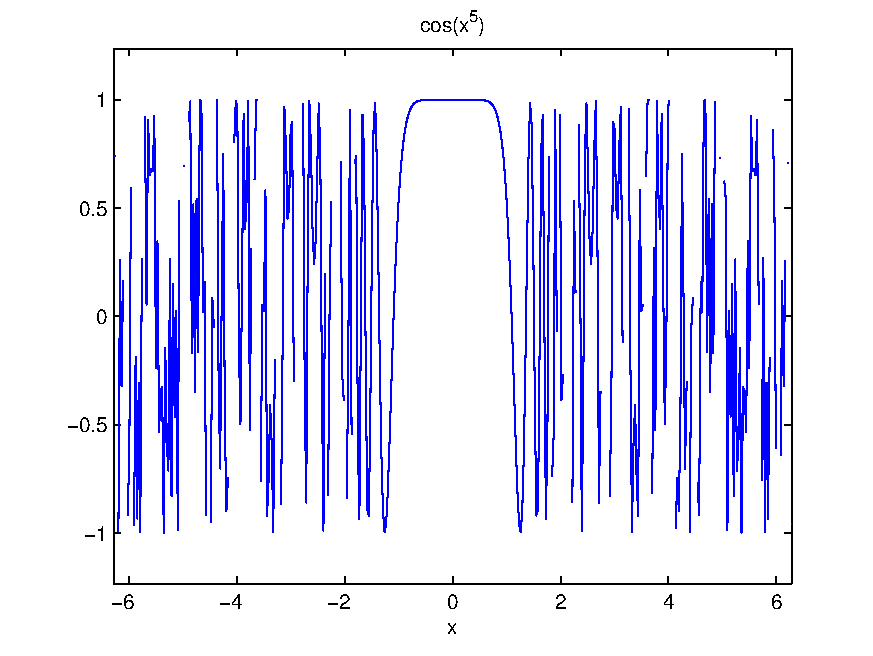
\psfig{figure=cosx5.eps,height=3in,width=3.2in}}}
%\centerline{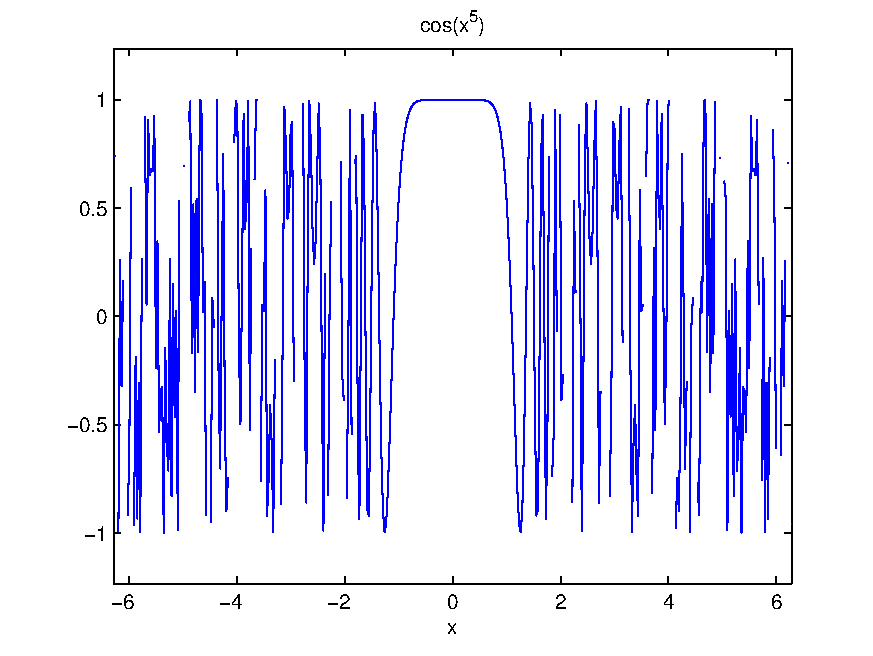
\includegraphics[width=0.6\textwidth]{cosx5}}
%\caption{Graph of $\cos(x^5)$ produced by the ezplot
%command. It is wrong because $\cos u$ should oscillate smoothly between
%$-1$ and $1$. The problem with the plot is that $\cos(x^5)$ oscillates
%extremely rapidly, and the plot did not consider enough points.}
%\label{fig:cosx5}
%\end{figure}
%
%%%%%%%%%%%%%%%%

\newpage

\subsection*{Functions of Two Variables and Partial Derivatives}

Since $f = \cos(x) + 3x^2$ and $g = \exp(-y^2)$ are functions of different variables,
their product is a function of two variables:
$$
k(x,y) = f(x) g(y) = ( \cos(x) + 3 x^2) \exp(-y^2)
$$
In \textsc{Matlab}, set
\begin{lstlisting}[frame=none,numbers=left]
k = f*g
\end{lstlisting}
To evaluate, we need to specify which value goes in which variable:
\begin{lstlisting}[frame=none,numbers=left]
subs(k,[x,y],[0,1])
\end{lstlisting}
To plot a symbolic function of two variables use:
\begin{lstlisting}[frame=none,numbers=left]
ezsurf(k)
\end{lstlisting}


If we want to differentiate a function with more than one variable in \textsc{Matlab}, we
must specify which variable we are differentiating with respect to:
\begin{lstlisting}[frame=none,numbers=left]
k1x = diff(k,x)
\end{lstlisting}
Here we have differentiated with respect to $x$. This is called the {\bf partial derivative} with respect to $x$ and
we use the symbol ${\displaystyle \frac{\partial k}{\partial x}}$ to denote it.
There is also a partial derivative with respect to $y$, i.e.\ ${\displaystyle \frac{\partial k}{\partial y}}$:
\begin{lstlisting}[frame=none,numbers=left]
k1y = diff(k,y)
\end{lstlisting}


To calculate a partial derivative by hand you differentiate as normal with respect to one variable, but
treat the other variables as if they were constants. For example if  $f(x,y) = x y^2$, then 
 $$
 \frac{\partial f}{ \partial x} = y^2 \quad \text{ and } \quad \frac{\partial f}{ \partial y} = 2 xy.
$$

\subsection*{Other useful symbolic operations}

\textsc{Matlab} allows you to do simple algebra. For instance:
\begin{lstlisting}[frame=none,numbers=left]
poly = (x - 3)^5
polyex = expand(poly)
polysi = simplify(polyex)
\end{lstlisting}
To find the symbolic solutions of an equation, $f(x) = 0$,
use:
\begin{lstlisting}[frame=none,numbers=left]
solve(f)
solve(g)
solve(polyex)
\end{lstlisting}
Another useful property of symbolic functions is that
you can substitute numerical vectors for the variables:
\begin{lstlisting}[frame=none,numbers=left]
X = 2:0.1:4;
Y = subs(polyex,X);
plot(X,Y)
\end{lstlisting}

\subsection*{New Notation}

\textsc{Matlab} recently expanded it notation for symbolic computations:
\begin{lstlisting}[frame=none,numbers=left]
syms x
f(x) = x^2;
f(2)
\end{lstlisting}
The function must be given as $f(x)$. If given as $f = x^2$ this will not work. Then we have to use 
\begin{lstlisting}[frame=none,numbers=left]
subs(f,2)
\end{lstlisting}
It works for multivariable functions also:
\begin{lstlisting}[frame=none,numbers=left]
syms x y a b
f(x,y) = x + 2*y;
f(a,b)
\end{lstlisting}

%%%%%%%%%%%%%%%%
\newpage
\subsection*{Exercises}
\begin{list}
{\arabic{chapter}.\arabic{exercise}}{\usecounter{exercise}}

\item Starting from \verb&mynewton& write a well-commented {\bf
    function} program \verb&mysymnewton& that takes as its input a
  symbolic function $f$ and the ordinary variables $x_0$ and $n$.  Let
  the program take the symbolic derivative $f'$. You will need to use the command
  \verb&subs& to obtain values of $f(x)$ and $f'(x)$. Test it on $f(x)=x^3-4$
  starting with $x_0=2$.  Turn in the program and a brief summary of
  the results.
  
  
\item Find a {\em complicated} function in an engineering or science
  textbook or website.  Make a well-commented {\bf script} program that defines 
  a symbolic version of this function and takes its derivative and
  indefinite integral symbolically (if possible). Plot the function on the domain that is relevant
  for the application. In the comments of the script
  describe what the function is and properly reference where you got
  it. Turn in your script and the plot.


\item Calculate all the partial derivative for the functions below. 
Do them by hand, then check them using the symbolic toolbox.

\hspace*{1cm} (a)  ${\displaystyle f(x,y) = \sqrt{xy} + x^2 \sin^2{y} }$   \qquad  \qquad  (b)  ${\displaystyle g(u,v) = \frac{uv}{u+v}}$.

\end{list}


%%%%%%%%%%%%%%%%%%%%%%%%%%%%%%%%%%%%%%%%%%%%%%%%%%%%%%%%%%%%%%%%%%%%%%

\chapter*{Review of Part I}
\addcontentsline{toc}{chapter}{Review of Part I}
\markboth{REVIEW OF PART I}{}



%%%%%%%%%%%%%%%%

\subsection*{Methods and Formulas}

%%%%%%%%%%%%%%%%

\subsubsection*{Solving equations numerically:}
\begin{description}
\item[$f(x) = 0$] --- an equation we wish to solve.
\item[$x^*$] --- a true solution.
\item[$x_0$] --- starting approximation.
\item[$x_n$] --- approximation after $n$ steps.
\item[$e_n = x_n - x^*$] --- error of $n$-th step.
\item[$r_n = y_n = f(x_n)$] --- residual at step $n$. 
Often $|r_n|$ is sufficient.
\end{description}

%%%%%%%%%%%%%%%%

\subsubsection*{Newton's method:}
\begin{equation*}
x_{i+1} = x_i - \frac{f(x_i)}{f'(x_i)}
\end{equation*}

%%%%%%%%%%%%%%%%

\subsubsection*{Bisection method:}
$f(a)$ and $f(b)$ must have different signs.\\
$x = (a+b)/2$\\
Choose $a = x$ or $b = x$, depending on signs.\\
$x^*$ is always inside $[a,b]$.\\
$e < (b-a)/2$, current maximum error.

%%%%%%%%%%%%%%%%

\subsubsection*{Secant method:}
\begin{equation*}
x_{i+1} = x_i - \frac{x_i - x_{i-1}}{y_i - y_{i-1}} y_i
\end{equation*}

%%%%%%%%%%%%%%%%

\subsubsection*{Regula Falsi} - a hybrid between secant and bisection methods.
\begin{equation*}
x = b - \frac{b - a}{f(b) - f(a)} f(b)
\end{equation*}
Choose $a = x$ or $b = x$, depending on signs.

%%%%%%%%%%%%%%%%

\subsubsection*{Convergence:}
Bisection is very slow.\\
Newton is very fast.\\
Secant methods are intermediate in speed.\\
Bisection and Regula Falsi never fail to converge.\\
Newton and Secant can fail if $x_0$ is not close to $x^*$.

%%%%%%%%%%%%%%%%

\subsubsection*{Locating roots:}
Use knowledge of the problem to begin with a reasonable domain.\\
Systematically search for sign changes of $f(x)$.\\
Choose $x_0$ between sign changes using bisection or secant.


%%%%%%%%%%%%%%%%

\subsubsection*{Usage:}
For Newton's method one must have formulas for $f(x)$ and $f'(x)$.\\
Secant methods are better for experiments and simulations.\\
Bisection and {\em Regula Falsi} are slower, but keep the root within the current bounds.

%%%%%%%%%%%%%%%%

\subsection*{\textsc{Matlab}}


%%%%%%%%%%%%%%%%

\subsubsection*{Commands:}

% \begin{lstlisting}[frame=none,numbers=left]
% v = [0 1 2 3]          % Make a row vector
% u = [0; 1; 2; 3]       % Make a column vector
% w = v'                 % Transpose: row vector --> column vector
% x = linspace(0,1,11)   % Make an evenly spaced vector of length 11
% x = -1:.1:1            % Make an evenly spaced vector, with increments 0.1
% y = x.^2               % Square all entries
% plot(x,y)              % plot y vs. x
% f = @(x) 2*x.^2 - 3*x + 1   % Make a function
% y = f(x)               % A function can act on a vector
% plot(x,y,'*','red')    % A plot with options
% Control-c              % Stops a computation.
% \end{lstlisting}

\verb&v = [0 1 2 3]& \dotfill Make a row vector.\\
\verb&u = [0; 1; 2; 3]& \dotfill Make a column vector.\\
\verb&w = v'& \dotfill Transpose: row vector $\leftrightarrow$ column vector \\
\verb&x = linspace(0,1,11)& \dotfill Make an evenly spaced vector of
                               length 11.\\
\verb&x = -1:.1:1& \dotfill Make an evenly spaced vector, with increments
                               $0.1$.\\
\verb&y = x.^2&  \dotfill Square all entries.\\
\verb&plot(x,y) & \dotfill plot y vs. x.\\
\verb&f = @(x) 2*x.^2 - 3*x + 1 & \dotfill Make an anonymous function.\\
\verb&y = f(x) &  \dotfill A function can act on a vector.\\
\verb&plot(x,y,'*','red')& \dotfill A plot with options.\\
\verb&Control-c & \dotfill Stops a computation.
%%%%%%%%%%%%%%%%

\subsubsection*{Program structures:}
\verb&for ... end& example:
\begin{lstlisting}
for i=1:20
   S = S + i;
end
\end{lstlisting}
\verb&if  ... end& example:
\begin{lstlisting}
if y == 0
    disp('An exact solution has been found')
end
\end{lstlisting}
\verb&while  ...  end& example:
\begin{lstlisting}
while i <= 20
   S = S + i;
   i = i + 1;
end
\end{lstlisting}
\verb&if  ... else ... end& example:
\begin{lstlisting}
if c*y>0
    a = x;
else
    b = x;
end
\end{lstlisting}

%%%%%%%%%%%%%%%%

\subsubsection*{Function Programs:}
\begin{itemize}
\item Begin with the word \verb&function&.
\item There are inputs and outputs.
\item The outputs, name of the function and the inputs must appear in the first line.\\
\hspace*{.5cm} i.e. \verb&function x = mynewton(f,x0,n)&
\item The body of the program must assign values to the outputs.
\item Internal variables are not visible outside the function.
\item A function program may not use variables in the current
                  workspace unless they are inputs.
\end{itemize}

%%%%%%%%%%%%%%%%

\subsubsection*{Script Programs:}
\begin{itemize}
\item There are no inputs and outputs.
\item A script program may use, create, change and even delete variables in the current
  workspace.
\end{itemize}

%%%%%%%%%%%%%%%%

\subsubsection*{Symbolic:}

% \begin{lstlisting}[frame=none,numbers=left]
% syms x y
% f = 2*x^2 - sqrt(3*x)
% subs(f,sym(pi))
% double(ans)
% g = log(abs(y))   % log is the natural logarithm
% h(x) = compose(g,f)
% k(x,y) = f*g
% ezplot(f)
% ezplot(g,-10,10)
% ezsurf(k)
% f1 = diff(f,x)
% F = int(f,x)      % indefinite integral (antiderivative)
% int(f,0,2*pi)     % definite integral
% poly = x*(x - 3)*(x-2)*(x-1)*(x+1)
% polyex = expand(poly)
% polysi = simple(polyex)
% solve(f)
% solve(g)
% solve(polyex)
% \end{lstlisting}
\verb&syms x y&\\
\verb&f = 2*x^2 - sqrt(3*x)&\\
\verb&subs(f,sym(pi)) &\\
\verb&double(ans)&\\
\verb&g = log(abs(y))& \dotfill \textsc{Matlab} uses \verb&log& for
                                     natural logarithm.\\
\verb&h(x) = compose(g,f)&\\
\verb&k(x,y) = f*g &\\
\verb&fplot(f)&\\
\verb&fplot(g,-10,10)&\\
\verb&ezsurf(k)&\\
%
\verb&f1 = diff(f,'x')& \\
\verb&F = int(f,'x')& \dotfill indefinite integral (antiderivative)\\
\verb&int(f,0,2*pi)& \dotfill definite integral\\
%
\verb&poly = x*(x - 3)*(x-2)*(x-1)*(x+1)&\\
\verb&polyex = expand(poly)&\\
\verb&polysi = simple(polyex)&\\
%
\verb&solve(f)&\\
\verb&solve(g)&\\
\verb&solve(polyex)&

